
\chapter{Introduction}
\label{ch:introduction}

Industries developing high integrity software are always looking for ways to
make their software safer. \gls{sil} are used to define a level of
risk-reduction provided by a safety-function. The highest \gls{sil}
\cite{siliso} which could be given to hardware or software system, as
given by the \gls{iec} \cite{iec} standard, is a SIL4. A SIL4 has a probability
of failure of between 0.0001 and 0.00001 \cite{IEC61508}, and although these
probabilities are very low, they are non-zero, and the upper bound of 0.000001
suggests a failure every once every 1,000,000 times on average, the outcome of
which can be catastrophic.

Software testing usually takes place when the program or a prototype has been
implemented. However by the time the product is fully implemented and errors are
caught it is expensive to go back to the planning stage to find solutions to
those bugs. Catching errors at an earlier stage of the project life cycle is
more time and cost effective for the whole project team.

One way of detecting errors at an early stage is by applying the use of \gls{fm}
at the design/specification stage of the project life cycle. The benefit of
using \gls{fm} is that they provide a means to symbolically examine the state
space of a design and establish a correctness that is true for all possible
inputs \cite{wifrm}. However due to the enormous complexity of systems these
days they are rarely used as they may not be feasible. 

\Gls{fm} come in different shapes and sizes. The \gls{asm} theory
\cite{Borger:2003:ASM:829603} is a state machine which operates on states or
arbitrary data structures. The B-method \cite{bmeth} is a formal method for the
development of program code from a specification in the \gls{asm} notation. Z
\cite{spiveyreferencemanual} is a specification language which is used for
describing computer-based systems. These are just a selection of various
\gls{fm} however there are a great deal more which are still applied to systems
today to add a degree of safety to certain high integrity products.

\Gls{specmod} and \gls{veri} may be done using different levels of rigour. Level
1 represents the use of mathematical logic to specify a system, level 2 uses a
handwritten approach to proofs and level 3 is the most rigorous application of
formal methods which uses theorem provers to undertake fully formal
machine-checked proofs. Level 3 is clearly the most expensive level and is only
practically worthwhile when the cost of making mistakes is extremely high
\cite{encyclopedia}.

The jump from Level 1 rigour to Level 3 rigour is very difficult, but in many
cases worthwhile. The purpose of this thesis is to introduce an toolset where
the large jump is broken up into multiple smaller jumps, allowing the level 3 of
rigour to be more accessible and thus more widely used. 

\section{Aims and Objectives}
This thesis presents a toolkit which analysis specifications for various degrees
of correctness and ultimately translates them into the theorem prover Isabelle.
The toolkit does this in a step by
step fashion. 
Our hypothesis is as follows:

\textbf{To what extent is breaking up the translation path from a
formal/semi-formal specification into a theorem prover, with various
safety checks along the way useful?}

To answer this hypothesis we have broken it down into the following research
questions:

\begin{enumerate}
    \item What and how many steps do we need to break up the translation path?
    \item Which steps can be automated to make it less labour-intensive for the user?
    \item What are the safety checks we can do along the way to a fully proven specification?
    \item Where could a toolkit such as \gls{zmath} be applied?
\end{enumerate}

The answer to the first research question is presented in chapter
\ref{ch:design} where the design of the toolkit is described and shows the six
steps needed to translate the specification. A high level description of the
automated tools are also described in chapter \ref{ch:design} and in particular
Figure \ref{fig:zmathflow}. Then the specific chapters on each aspects (chapters
\ref{ch:zcga} to \ref{chap:gpsa2isa}) describe in detail the automated
components, which gives us an answer to the second research question. We
describe the possible safety checks in the background chapter (chapter
\ref{ch:background}) but incorporate particular safety checks to help with the
translation in chapter \ref{ch:skeletons}. We presented the toolkit
to various industry experts from different domains and recorded their comments
in chapter \ref{ch:evaluation}, which answers our final research question.

\section{Contributions}

The focus of this thesis presents \gls{zmath}, which is an adaptation of the
MathLang framework \cite{newmathlang}, \cite{wtt}. Z is a formal notation to
describe the functions and layout of a system (more details found in section
\ref{sec:theznotation} of this thesis). \Gls{zmath} is a collection of tools
which assist the user in checking the correctness of formal specifications, and
also assist users by partially automating the translation of the specification
into a theorem prover. There are aspects of formalisations and proofs
contributed in this thesis however they are smaller parts which come from the
tool support built to translate specification into Isabelle. We summaries the
contributions of this thesis in the following list:

\begin{enumerate}
\item Staged an approach to translating semi-formal and formal specifications
into Isabelle with automatic assistance (described in chapter \ref{ch:design}
and entire thesis).
\item Built a collection of tools to enable a step by step approach for Z
specifications (includes ZCGa implementation in chapter \ref{ch:zcga}, ZDRa implementation in
chapter \ref{ch:zdra} and further aspects in chapters \ref{ch:skeletons},
\ref{chap:gpsa2isa} and \ref{ch:interface}).
\item Formalised and proved properties on a number of examples of Z
specifications (described in chapters \ref{ch:fullexample}, \ref{ch:evaluation}
and in \cite{mathlangexamples}).
\item Demonstrated and evaluated the performance of the tool set on a convincing
set of examples (described in chapter \ref{ch:analysis} and \ref{ch:evaluation}).
\end{enumerate}

\subsection{Staged an approach to translating semi-formal and formal specifications into Isabelle with automatic assistance.}

Translating specifications into theorem provers has been shown to be a great
difficult task \cite{johnharrisonslides}. Not everyone on the software project
team will know how to computerise specifications. The main contribution this
thesis presents a tool support to assist in the translating formal
specifications into theorem provers. The \gls{zmath} toolset has been designed
for individuals who have no or little expertise in the chosen theorem prover. It
is broken up so that each step in the path checks for some form of correctness
of the specification. The checks become more and more rigorous the further one
goes along the path.

Our approach can also translate partially formal specifications into theorem
provers. That is specifications written in natural language which is on it's way
to becoming formalised. The line belows shows a semi-formal sentence taken from
a specification describing a clock.

\begin{verbatim}
A clock tells the time:nat.
Time is on going therefore time' < time
\end{verbatim}

Not only does our new approach assist with translating the text but it can also
performs the various checks of rigor along the way. For example, the grammatical
correctness of this example can be checked (see \gls{zcga} chapter
\ref{ch:zcga}) without it needing to be fully formalised. The documents
rhetorical correctness (see \gls{zdra} chapter \ref{ch:zdra}) can also be
checked without the need for the document to be fully formal. \Gls{zmath} is one
framework made up of many smaller tools to deliver it's main aim, which is to
computerise a system specification. The \gls{zmath} framework has stemmed from
the \gls{math} framework \cite{mathintomizar} and has been adapted to work for Z
specifications.

\subsection{Built tools to enable this approach.}

Another contribution of this thesis is the tools which we have built in order to
check for various degrees of correctness and to produce documents which could be
used for the system in question.

Again the innovation in this research is that the tools can act upon system
specifications which have been partially formalised. Some examples of the tools
are listed below:

\begin{itemize}
\item A tool to check the grammar of the system specification.

\item A tool which check the rhetorical layout of the specification.

\item A tool which produces documents to order the chunks of the specification.
\end{itemize}

The first tool to check's the grammar of the document. To do this the user first
annotates the specification with grammatical labels and then uses the automatic
grammar checker to check the labels. These labels are known as
`\emph{categories}' and describe the elements found in formal specifications
such as `\emph{terms}', `\emph{sets}' and `\emph{expressions}'. 

The second tool checks the documents rhetorical correctness. That is, it checks
for any loops in the reasoning. This tool can be used on a specification which
is written formally, semi-formally or completely in natural language. The
rhetorical checker chunks part of the text together and describes the
relationships between each chunk. Similar to the previous tool, the user labels
the text and then uses the program to check for any loops in the reasoning of
the document. The chunks include sections which change the state of the
specification, or output a message etc.

One of \gls{zmath} tools is able automatically produce documents which can be
used to analyse the system. These documents are simple to understand by
stakeholders of the project and can be used to describe to clients, developers,
managers etc. 

\subsection{Formalised and proved properties on a number of examples of Z specifications.}

A third contribution given in this thesis is that we have formalised and
translated Z specifications into the theorem prover Isabelle and checked the
sanity of these specifications. The sanity properties (described in the next
section) were automatically generated by the \gls{zmath} toolkit and we have
manually proved the properties in Isabelle.

In some examples we have added extra properties (such as the birthdayBook
example) to show what other properties may be proved in Isabelle. Although these
properties have not been automatically generated, they may be of some importance
to some users. Other properties which could be manually inputted are described
in section \ref{subsec:propertiestoprove}.

%is a formal view on some of \gls{zmath}'s tools (shown in chapter
%\ref{ch:formal}). The grammatical correctness checker for mathematics has
%already been formalised in previous research. Since the formal specification
%grammar checker is an adaptation of the mathematics one, we have presented a
%formal view on the adaptation. Rules and properties for the Document Rhetorical
%aspect have been implemented (see table \ref{tab:relationsallowed} in chapter
%\ref{ch:zdra}). We have identified these rules in order to reason with and show
%certain properties about them in chapter \ref{ch:formal}. Based on ideas from
%\cite{zengfirstyear}, we develop our own formalisation of the document
%rhetorical checking program as well as the products it automatically produces. 
%
%We give a formal view on the dependency and goto graphs using various
%definitions to describe the relations between nodes and edges. We also give
%examples of the nodes and edges of an annotated text and describe its
%equivalent nodes and edges in the dependency and goto graphs. The formal
%definitions from \cite{zengfirstyear} have been used to construct the adapted
%definitions and properties for the document rhetorical aspect and graphs
%presented in this thesis.

\subsubsection{Automatically generated properties to check the sanity of the specifications.}
We have designed and
implemented a tool which automatically generates safety properties to prove in
Isabelle syntax. The properties used in the examples are in the class of sanity
checks in which the state invariants of the system specification are checked
against all the state changing schemas.

There are many other properties one can check in systems such as properties
across specifications, required properties of a single specification etc (see
section \ref{subsec:propertiestoprove} in chapter \ref{ch:background}).
However in this thesis we have supplied a formal definition for the sanity
checks of Z specifications and implemented it in our tool so that it is
automatically added during the translation.


\subsection{Demonstrated and evaluated the performance of the tool set on a convincing set of examples.}

Another contribution this thesis presents is our approach shown on a convincing
set of examples. We have used our approach on the following specifications

\begin{tabular}{l l}
$\bullet$ BirthdayBook \cite{spiveyreferencemanual} & $\bullet$ Vending Machine
\cite{pp} \\
$\bullet$ Clubstate \cite{essenceofz} & $\bullet$ Clubstate2 \cite{essenceofz}
\\
$\bullet$ ModuleReg \cite{essenceofz} & $\bullet$ ProjectAlloc \cite{essenceofz}
\\
$\bullet$ TelephoneBook & $\bullet$ Timetable \cite{essenceofz} \\
$\bullet$ VideoShop \cite{essenceofz} & $\bullet$ Steamboiler
\cite{steamboilerslides} \\
$\bullet$ A specification which fails ZCGa & \\
$\bullet$ A specification which fails ZDRa & \\
$\bullet$ Autopilot (A semi formal Specification) \cite{Butler96} & \\
$\bullet$ The ZCGa type checker & \\
\end{tabular}

We have analysed the complexity of each of these specifications and shown in
detail a few case studies of translating these specification using the toolkit
of \gls{zmath}. We have discussed how the complexity affects the translation and
given details on lines of code in each specification, amount of different
environments for each specification and the amount of annotations needed for
each specification.

\section{How far does the automation go?}

Figure \ref{fig:timeline} shows a diagram showing how far one can automate a
specification using automated \gls{zmath} and Isabelle tools. \Gls{zmath} is a
toolset which assists the user in translating and proving a specification (going
from left to right). There are also other automating tools within Isabelle which
also assist the user with proving specifications (going from right to left) in
the diagram.

\begin{figure}[H]
 \begin{center}
 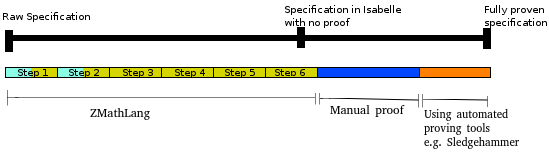
\includegraphics [scale=0.75]{Figures/Design/timeline2.png}
 \caption{How far can one automate a specification proof.}
 \label{fig:timeline}
\end{center}
\end{figure} 

In figure \ref{fig:timeline} we show how far the user can get with automation
and how much work is still needed to get the full proof \footnote{Full
proof/full correctness in reference to completing sanity checks of the
specification. Full correctness can be variable depending on the users choice.
This is further discussed in chapter \ref{ch:evaluation}.}. \Gls{zmath} requires
user input for the first two steps (\gls{zcga} and \gls{zdra}) however the rest
up to step 6 is automated.

The black line shows the path going from a raw specification to a fully proven
specification with a milestone in the middle, which signifies when a
specification has been translated into Isabelle syntax but has no properties or
proof. \Gls{zmath} takes the user a little past this milestone as the toolset
also generates properties to check the specification for consistency (see
section \ref{sec:proofobl}). These properties are added to the specification
during step 3 and continued throughout the translation. It is important to note
that the \gls{zmath} toolkit adds these properties to the translation but does
not prove them. That is why the rest of the \gls{zmath} path may require
external user input (dark blue) to complete the path. However, the \gls{zmath}
toolkit does assist the user in the translation past the halfway milestone on
the diagram.

We have created the \Gls{zmath} toolkit which assist the user from the
specification to full proof however there is also ongoing research on proving
properties from the theorem prover end. We have highlighted that
\gls{zmath} only gets the user so far in their proof however they are free to
use external automated theorem provers such as sledgehammer in completing their specification proof
if they so wish.

Even external automated theorem provers have their limitations. For example, the
user can use the Isabelle tool `\emph{sledgehammer}' to assist in solving
proofs, but not all can be solved by this technique. The sledgehammer
documentation advises to call `\emph{auto}' or `\emph{safe}' followed by
`\emph{simp\_all}' before invoking sledgehammer. Depending on the complexity of
ones proof, these sometimes may prove the users properties on their own, other
times it may not and the user will still need to invoke sledgehammer to reach
their goal. Sledgehammer itself is a tool that applies \gls{smt} solvers on the
current goal e.g. Vampire\cite{vampire}, SPASS \cite{fmintrol} and E \cite{e}. We
use sledghammer as a collective, to describe all the \gls{smt} solvers it covers
\cite{sledgehammer}. However, there
still doesn't exist an automated proving tool which covers \textbf{all} proving
techniques. Therefore some user input will be required for more complex proofs.

\section{Outline}

In chapter \ref{ch:background} we begin describing the origins of \gls{math},
its success and where it has been used so far. We then describe Z specifications
and the tools available for it so far.

%In chapter \ref{ch:Contributions}, We highlight the contributions of this
%thesis as well as outline the basic idea of \gls{zmath}, how the original
%\gls{math} method has been adapted to perform with Z specifications and how
%this method is different to others previously described.

Chapter \ref{ch:zcga} provides more in depth details of the first contribution
of this thesis. The weak types which have been created are presented as well as
how they work together with weak typing rules. The categories which have been
extracted from the weak types are presented and examples are given on how these
categories correspond to Z specifications. Examples are given for all the weak
types, and categories for Z specification. The weak type checker, which is
implemented in \texttt{Python} \cite{Python}, is thoroughly described and
details of how the tool can be used are given.

Chapter \ref{ch:zdra} highlights another contribution of this thesis. An
explanation of rhetorical correctness for a specification is given. Instances
and how they relate to each other are described as well as how a user can
annotate these facts into a Z specification. Examples are given for all
relations and instances, and rules are provided of what relations are allowed.
An outline of the \gls{zdra} checker is given, along with explanations of
various error and warning messages. A general explanation of the dependency and
GoTo graphs is also given.

Chapter \ref{ch:skeletons} describes the different skeletons which can be
automatically generated if the specification is \gls{zdra} correct. A detail
explanation of how a general proof skeleton can be created from the GoTo graph
is given along with the algorithm which creates it. 

Chapter \ref{chap:gpsa2isa} summarises the path of how the general proof sketch
can be used to generate an Isabelle skeleton of the specification. Details of
how the Isabelle skeleton can be filled in using the \gls{zcga} annotated
specification is also shown in this chapter. A demonstration of how we can use
this filled in Isabelle skeleton to get a full proof is also described. It also
gives formal definitions of the \gls{zdra} correctness checker, dependency
graphs and GoTo graphs. We prove various properties about the \gls{zdra}. We
give examples of how each of these aspects can be represented in a formal
manner. The algorithm which creates the dependency and GoTo graphs is given and
explained.

In chapter \ref{ch:interface} we give an overview on the user interface for
\gls{zmath} and we explain how one can use \gls{zmath} on Z specifications.
Explanations of how to use each aspect are given via examples and screen shots.
The tables of output messages which a user can receive are highlighted and
explained.

Chapter \ref{ch:fullexample} goes through one entire specification (modulereg
specification \cite{essenceofz}) along the \gls{zmath} route. Each aspect is
clearly highlighted and explained to the reader giving hints and tips along the
way. Other examples are found in the appendix, however they are only taken along
the \gls{zmath} route without any commentary.

In chapter \ref{ch:analysis} we consider 2 specification examples which have
been proven in a theorem prover using a single step, and compare them with the
same specification examples which have been proven in multiple steps using
\gls{zmath}. We give a table of comparison explaining the amount of expertise
required, type of input and lines of proofs and lemmas. We explain and compare
the type of expertise required for each of the specification examples and how
doing the proof in one step compares against or multiple steps.

Chapter \ref{ch:evaluation} evaluates the \gls{zmath} toolkit. Gives details on
the complexity of the specifications we have translated and goes through some
specification case studies.

Finally, a conclusion is presented in chapter \ref{ch:conclusion} which
summarises the contributions made in this thesis. The limitations of this
research and potential areas of future research are also discussed.
